\section{Results - Curriculum Reinforcement Learning} \label{sec: Results - Curriculum Reinforcement Learning}

In this final results section, we demonstrate the role of Curriculum Learning in enhancing the RL agent’s training process. By gradually increasing the complexity of the environment, we show how CL contributes to improved learning efficiency and overall performance. Obtained results are described in the following fashion:
First subsection describes a setting of a baseline results to verify the possible improvements that can be achieved with CL. Second and third subsections provide an understanding on the CL parameters selection. Fourth subsection describes the obtained results, while the fifth gives a comparison of the best achieved systems to the baseline. 

\todo[inline, disable]{Chance all those points to subsections (as below) - addressed}
\subsection{Setting up a baseline}

Before proceeding with the analysis, it is essential to establish baseline results for the continuous RL PPO method, without enhancements from Curriculum Learning. This provides a point of reference to assess how much CL can improve performance. For this we have conducted tests using the system parameters presented in the Table~\ref{tab:hyperparameters} and~\ref{tab:env_params} for systems with 1 to 3 links. For each system, 10 distinct simulation cases were executed to account for variability in control due to different initial conditions. The baseline is determined by measuring the training timesteps required for success, focusing primarily on the mean and median values, which serve as the key performance indicators. Additionally, the minimum and maximum values provide insight into the range of results across cases. These metrics allow us to assess the general performance of PPO in continuous action space. Table~\ref{tab: baseline statistics for PPO in continuous action space} summarizes the results for the RL training using the PPO algorithm in continuous action space. The results are presented for systems with 1, 2, and 3 links.

\begin{table}[ht]
	\centering
	\caption{Baseline results of using PPO algorithm in continuous action space for 1 to 3 link pendulum systems}
	\begin{tabular}{@{}lccccc@{}}
		\toprule
		\textbf{System} & \textbf{Successful cases} & \textbf{Mean} & \textbf{Median} & \textbf{Minimum} & \textbf{Maximum} \\ \midrule
		\textit{1-link} & 10 & 26168 & 25600 & 24320 & 32000 \\
		\textit{2-link} & 7 & 48055 & 49152 & 38400 & 55296 \\
		\textit{3-link} & 5 & 278937 & 288768 & 194560 & 319488 \\ \bottomrule
	\end{tabular}
	\label{tab: baseline statistics for PPO in continuous action space}
\end{table}

As indicated in Table~\ref{tab: baseline statistics for PPO in continuous action space}, the results show a clear progression in training time as the system complexity increases from 1-link to 3-link. The 1-link system requires the least number of timesteps on average to reach successful training, while the 3-link system exhibits significantly higher values, with a mean training time nearly 10 times longer than the 1-link system. This demonstrates that as the system complexity increases, the training duration grows substantially, making it harder for the PPO algorithm to converge quickly.
The primary goal of introducing CL enhancement is to accelerate the training process and potentially make the system more robust to various initial conditions. By progressively increasing the difficulty of the tasks during training, we aim to reduce the number of timesteps required for convergence. To further explore the impact of CL, the next step focuses on selecting the appropriate CL implementation parameters, dividing the research into well-defined steps. 

\subsection{Selection of a decay function} 

At first, we shall determine which decay type is specifically the most performing for our particular task of pendulum stabilization. For this we have tested all previously described decay functions in subsection~\ref{subsec: Curriculum learning implementation} on a single pendulum system. With 150 runs per decay function of 5 initialization cases we use control values vector of the form 
\(\begin{bmatrix} 1 & n \end{bmatrix}\), where \(n = 2, 4, 6, 8, 10\) and decay steps $k$ values are selected as \(k = 5000, 6000, \ldots, 10000\) to evaluate the performance across different control parameters\todo[inline, disable]{All this is unclear. What is "control values matrix" and "decay steps vector"? Were they defined and are they needed to explain the task? To me this representation is redundant, due to those zeros (which are implicitly implied by task definition). Explanation of it traces back to Section 2. - updated: changed from matrix to vector and added a better description in Section 2}. The results are presented in a form of a bar plot, which shows the number of agent successes for the whole dataset. See Figure~\ref{fig: decay types comparison}.  

\begin{figure}[h]
	\centering
	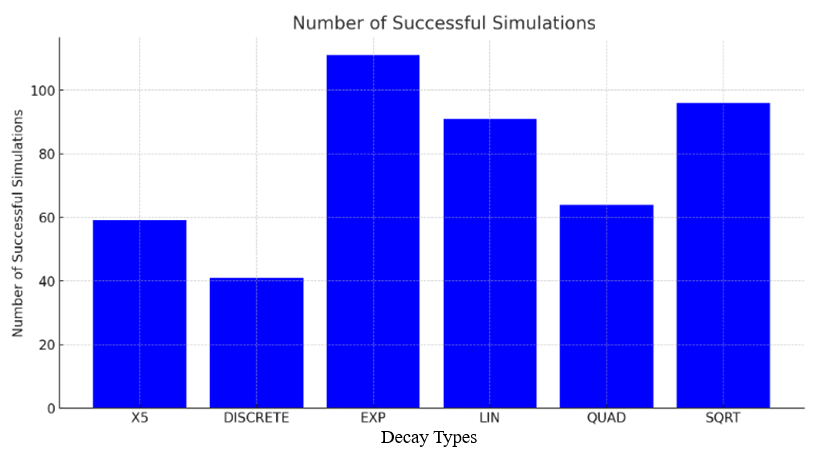
\includegraphics[width=12cm]{Figures/decay_types_results_comparison.png}
	\caption{Simulation results for decay types analysis. Each bar plot represents the value of successfully trained cases out of 150 in total per decay function.}
	\label{fig: decay types comparison}
\end{figure}

The exponential decay function provides the best results of having 74\% success rate across the dataset and therefore will be considered as the main function used in our next analysis. 

\subsection{Selection of a decay factor} 

For the selection of the decay factor, we have performed an extensive analysis using a double pendulum system. The control values were set as \(\begin{bmatrix} 1 & n & n \end{bmatrix}\), where \(n = 1, 2, \ldots, 10\). For each unique combination of control values, decay steps, and decay factors, we ran 10 trials, each corresponding to a different set of initial conditions for the system to begin training. This approach ensured the reliability and robustness of the results. In total, we analyzed four decay factors: 0.005, 0.01, 0.05, and 0.5, resulting in 5600 unique cases across the experiments.\todo[inline, disable]{It's unclear (and irrelevant) what are "lines of result". Rewrite. Provide, e.g., number of cases or similar measure. - described}. The objective of this analysis was to determine the optimal decay factor for maximizing the system's learning performance.
The output metric used for comparison included the value of training timesteps. This metric provide insight into how efficiently the system is able to solve tasks within the corresponding timesteps.

\begin{figure}[h] 
	\centering 
	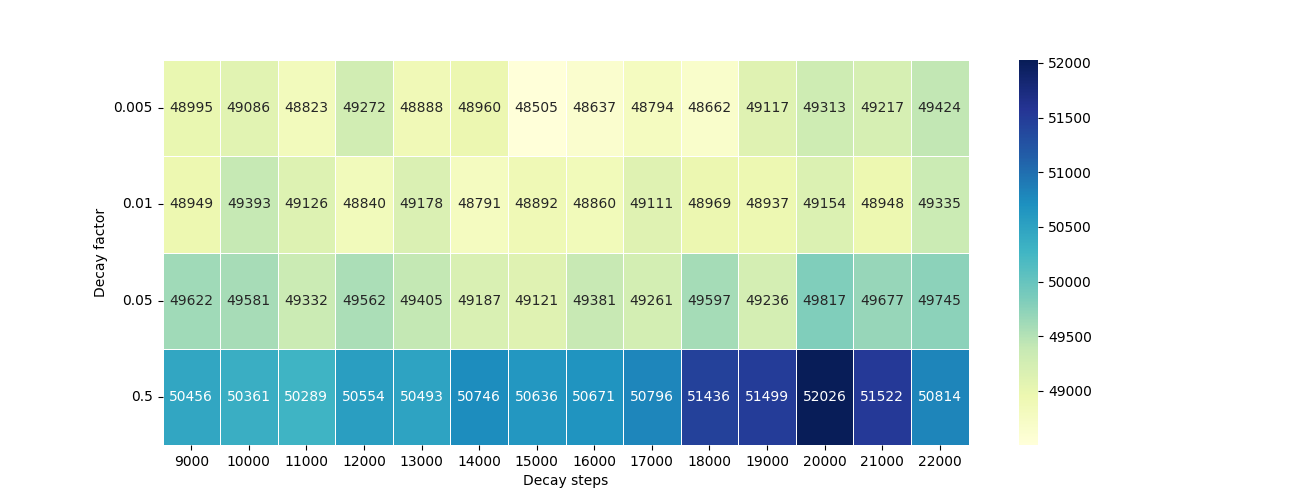
\includegraphics[width=15cm]{Figures/MaxSuccessfulTestsTimesteps_heatmap.png} 
	\caption{Heatmap showing the impact of different decay factors on the number of successful tests and timesteps. The decay factor 0.005 consistently performs best in terms of minimizing timesteps.} 
	\label{fig: decay factors comparison}
\end{figure}

As shown in Figure~\ref{fig: decay factors comparison} decay factor 0.005 consistently results in the lowest timesteps across all combinations of control values and decay steps. This indicates that the system converges faster and more efficiently with a decay factor of 0.005 compared to the other decay factors. The smaller the timesteps, the faster the system is able to learn, making 0.005 the most optimal choice for our training setup.

\subsection{CL enhancement: overview} 

% description of the results - TO-DO

\begin{figure}[h!]
	\centering
	\begin{subfigure}[t]{0.48\textwidth}
		\centering
		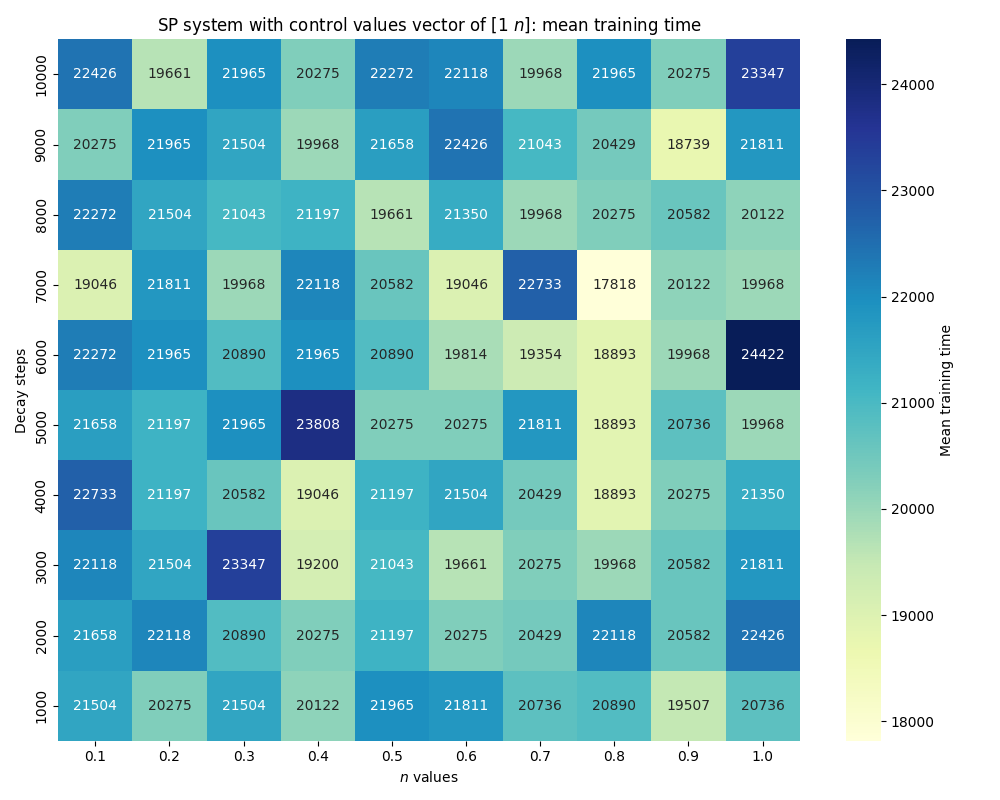
\includegraphics[width=\textwidth]{Figures/SP_cv_01_to_1.png}
		\caption{1-link. Control values varied from 0.1 to 1, decay steps range from 1000 to 10000}
	\end{subfigure}
	\begin{subfigure}[t]{0.48\textwidth}
		\centering
		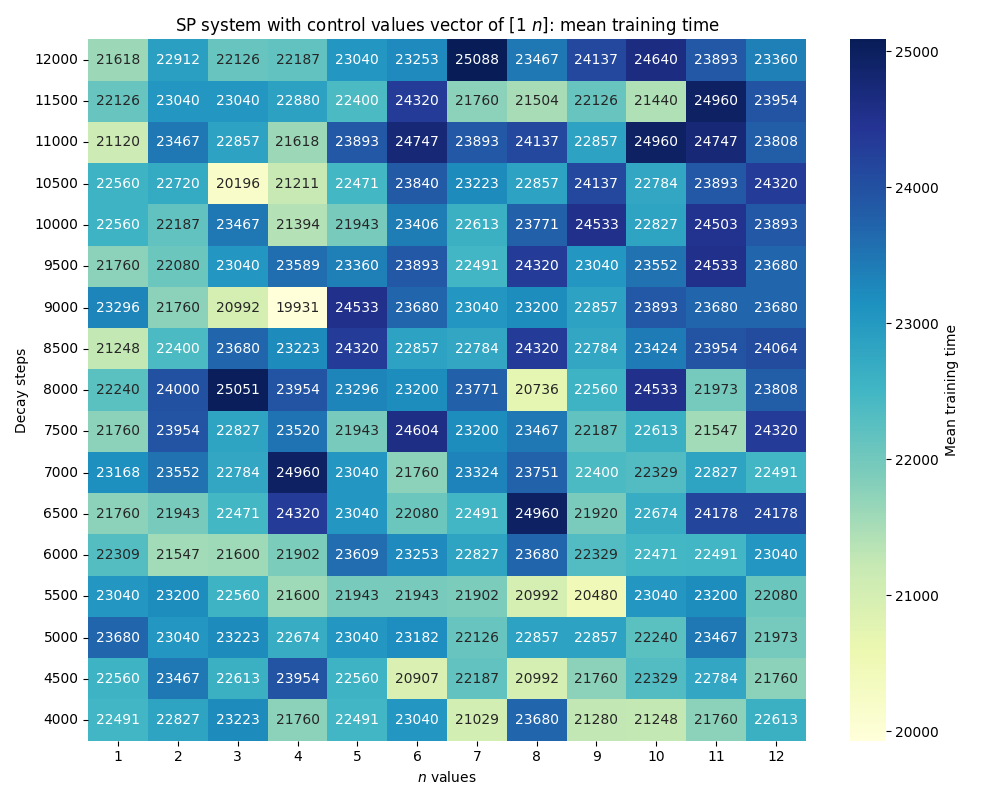
\includegraphics[width=\textwidth]{Figures/SP_cv_1_to_12.png}
		\caption{1-link. Control values varied from 1 to 12, decay steps range from 4000 to 12000}
	\end{subfigure}
	\begin{subfigure}[t]{0.48\textwidth}
		\centering
		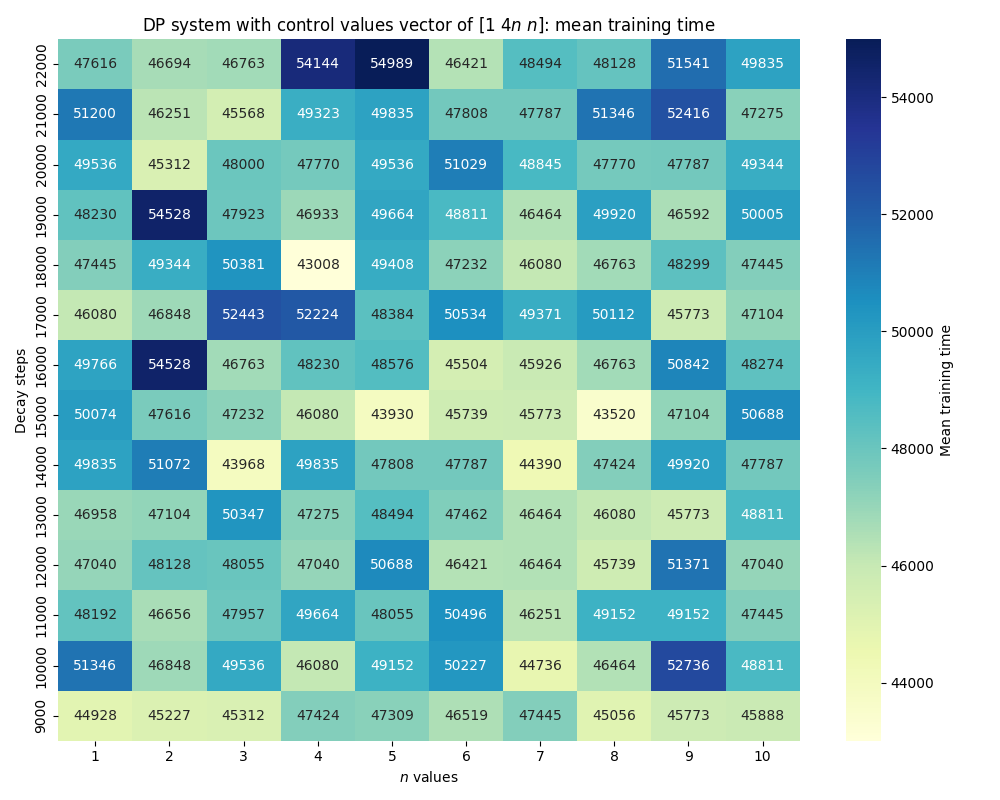
\includegraphics[width=\textwidth]{Figures/DP_1_4n_n_heatmap_mean.png}
		\caption{2-link. $n$ value varied from 1 to 10, decay steps range from 9000 to 22000}
	\end{subfigure}
	\begin{subfigure}[t]{0.48\textwidth}
		\centering
		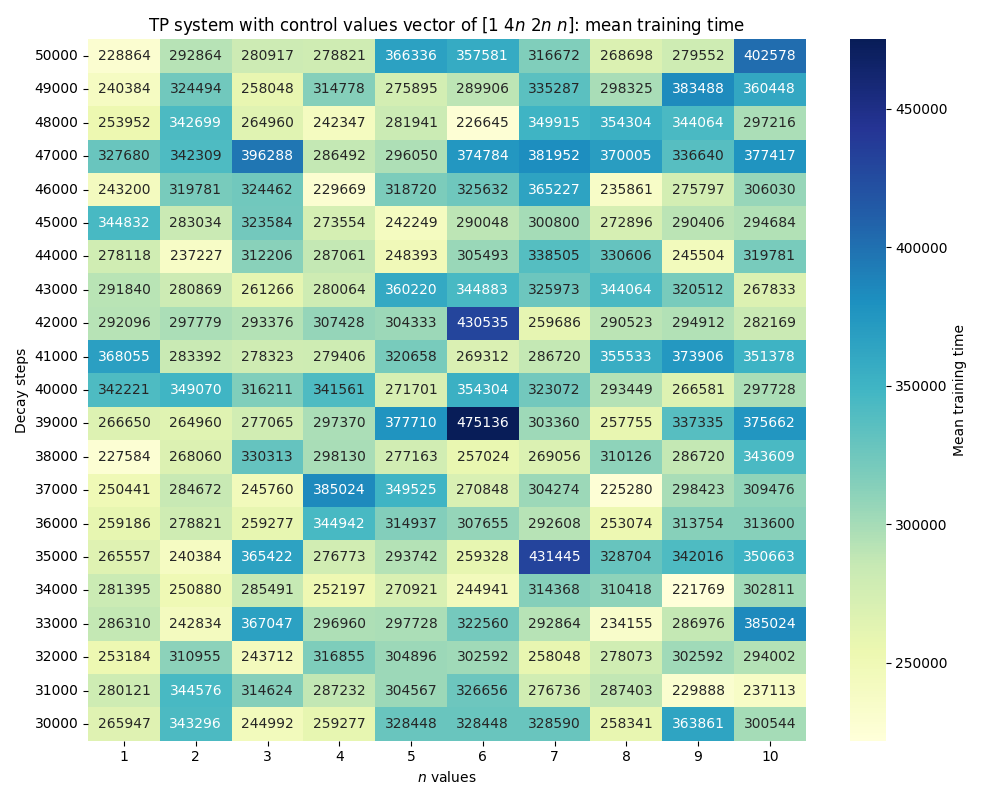
\includegraphics[width=\textwidth]{Figures/TP_1_4n_2n_n_heatmap_mean.png}
		\caption{3-link. $n$ value varied from 1 to 10, decay steps range from 30000 to 50000}
	\end{subfigure}
	
	\caption{Heatmaps with mean system training time for 1-link (a), (b), for 2-link (c) and 3-link (d) systems under various control values and decay steps}
	\label{fig: CL heatmaps}
\end{figure}

% slight transition to the best model evaluation - TO-DO

\subsection{CL enhancement: evaluation within the baseline}

The next step in our analysis involves the development of a control value decay scheme to assess its influence while varying decay steps. For the single pendulum system, the control values matrix is maintained as \(\begin{bmatrix} 1 & n \\ 0 & 0 \end{bmatrix}\), since the simplicity of the system allows for efficient training without requiring significant constraints on movement. Experiments were conducted by varying $n$ from 0.1 to 1 (step size of 0.1), and from 1 to 12 (step size of 1). Decay steps ranged from 1000 to 12000, with increments of 1000. 
For the double pendulum system, the control scheme was set as \(\begin{bmatrix} 1 & c \cdot n & r \cdot n \\ 0 & 0 & 0 \end{bmatrix}\), where $c$ and $r$ represent extension coefficients used to observe the effects of pendulum link constraint magnitudes on the results and are varied over the set \({1, 2, 4, 8}\), while \(n = 1, 2, \ldots, 10\). Decay steps were varied between 9000 and 22000, with an increment of 1000. 
For the triple link system, the control scheme used was \(\begin{bmatrix} 1 & 4n & 2n & n \\ 0 & 0 & 0 & 0 \end{bmatrix}\), where \(n = 1, 2, \ldots, 10\). This configuration required stronger restrictions on the first link due to its responsibility in bearing the mass of the subsequent links. The decay steps were varied between 30000 and 50000, with increments of 1000.
The evaluation of results was performed across cases within each unique combination of control values and decay steps, rather than across the entire control scheme. This is due to the CL implementation, which focuses on enhancing training efficiency where the key factor is to find the optimal combination of values to facilitate faster and more robust learning in the system. To determine the best-performing combination of control values and decay steps, we concentrated on three primary factors: number of successful cases in each combination, mean and median values of training time across cases. For the single and double pendulum systems, a successful case was defined as achieving 50 out of 50 successful tests. For the triple pendulum system, due to its higher complexity, the threshold for success was set at 70 out of 100 tests passed. This adjustment reflects the increased difficulty of achieving full success for the triple link system. The results are shown in the Table~\ref{tab: CL results}.\todo[]{Explain briefly what was the measure to select the best performing scheme.}

\begin{table}[ht]
	\centering
	\caption{CL enhancement: best results for 1 to 3 link pendulum systems}
	\begin{tabular}{@{}lccccc@{}}
		\toprule
		\textbf{System} & \makecell{\textbf{Best performing}\\ \textbf{schemes}} & \makecell{\textbf{Successful}\\ \textbf{cases}} & \makecell{\textbf{Decay}\\ \textbf{steps}} & \textbf{Mean} & \textbf{Median} \\ \midrule
		\textit{1-link} & \(\begin{bmatrix} 1 & 0.8 \\ 0 & 0 \end{bmatrix}\) & 10 & 7000 & 17817 & 18432 \\ \midrule
		\textit{2-link} & \(\begin{bmatrix} 1 & 20 & 5 \\ 0 & 0 & 0 \end{bmatrix}\) & 10 & 15000 & 43929 & 43008 \\ \midrule
		\textit{3-link} & \(\begin{bmatrix} 1 & 16 & 8 & 4 \\ 0 & 0 & 0 & 0 \end{bmatrix}\) & 10 & 30000 & 233676 & 216064 \\ \bottomrule
	\end{tabular}
	\label{tab: CL results}
\end{table}

The results in Table~\ref{tab: CL results} demonstrate the effectiveness of the best-performing control schemes across the three systems, with all systems achieving 10 out of 10 successful cases.\todo[]{Discuss the steps as well. Irrespective they are better or not.} These results highlight the robustness of the implemented Curriculum Learning in reducing training times while maintaining high success rates, even as system complexity increases.
To gain further insights into how the variations in control schemes and decay steps influenced the training times, we present a series of heatmaps showed on Figure~\ref{fig: percentage heatmaps for 1- to 3- link systems using CL} (a) to (f). The percentage change in both mean and median training times for each pendulum system is visualized, offering a clear depiction of the impact of CL enhancements across different cases.

\begin{figure}[h!]
	\centering
	\begin{subfigure}[t]{0.32\textwidth}
		\centering
		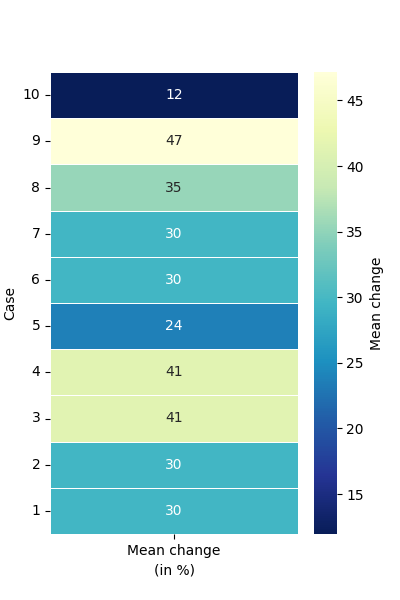
\includegraphics[width=\textwidth]{Figures/SP_mean_heatmap_percentage.png}
		\label{fig: SP_mean}
		\caption{}
	\end{subfigure}
	\hfill
	\begin{subfigure}[t]{0.32\textwidth}
		\centering
		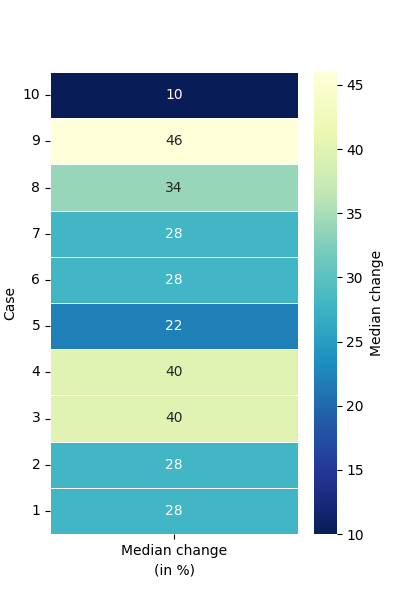
\includegraphics[width=\textwidth]{Figures/SP_median_heatmap_percentage.png}
		\label{fig: SP_median}
		\caption{}
	\end{subfigure}
	\hfill
	\begin{subfigure}[t]{0.32\textwidth}
		\centering
		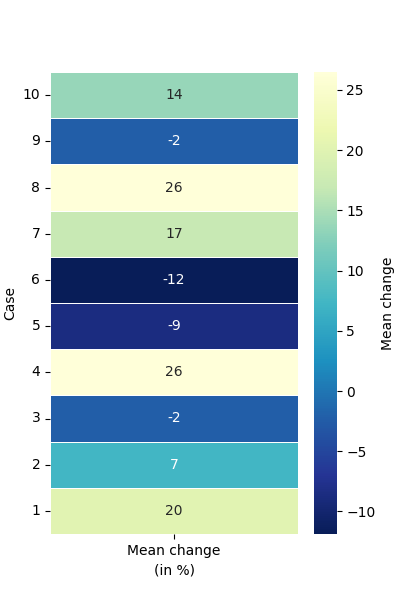
\includegraphics[width=\textwidth]{Figures/DP_mean_heatmap_percentage.png}
		\label{fig: DP_mean}
		\caption{}
	\end{subfigure}
	
	\vspace{0.2cm}
	
	\begin{subfigure}[t]{0.32\textwidth}
		\centering
		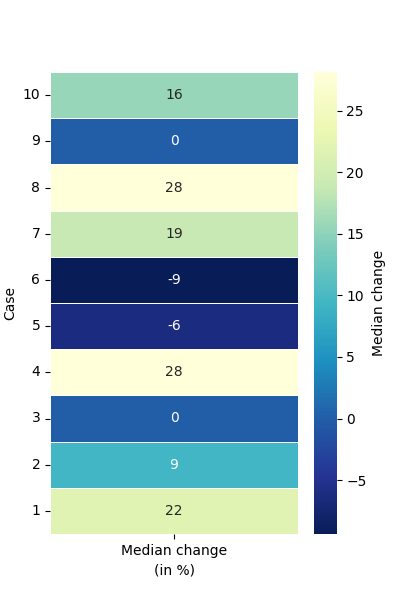
\includegraphics[width=\textwidth]{Figures/DP_median_heatmap_percentage.png}
		\label{fig: DP_median}
		\caption{}
	\end{subfigure}
	\hfill
	\begin{subfigure}[t]{0.32\textwidth}
		\centering
		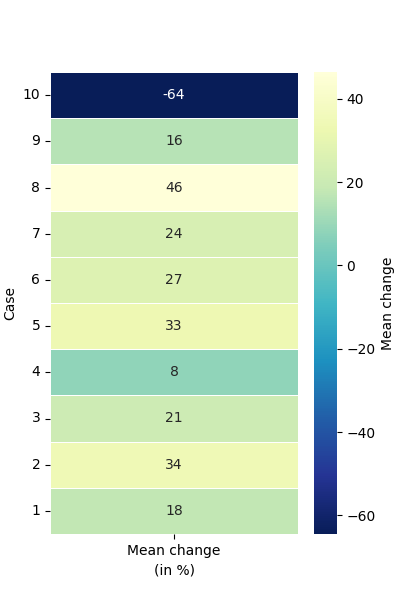
\includegraphics[width=\textwidth]{Figures/TP_mean_heatmap_percentage.png}
		\label{fig: TP_mean}
		\caption{}
	\end{subfigure}
	\hfill
	\begin{subfigure}[t]{0.32\textwidth}
		\centering
		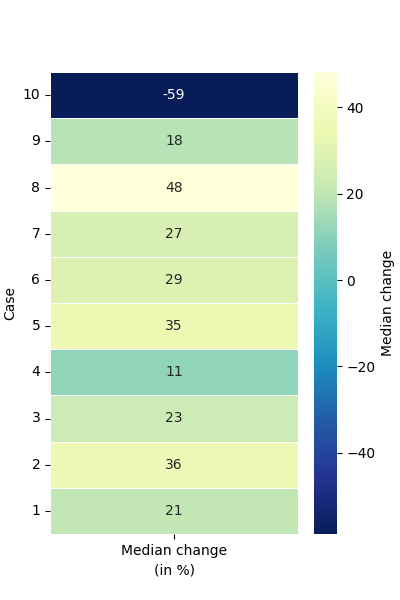
\includegraphics[width=\textwidth]{Figures/TP_median_heatmap_percentage.png}
		\label{fig: TP_median}
		\caption{}
	\end{subfigure}
	
	\caption{Mean and median training time change per cases for 1- to 3- link pendulum systems using CL enhancement.\todo[inline]{Denote with systems are shown in plots a to f. Are those training times or cases? Explain what is shown and what is expected - are the positive or negative numbers the "good" ones?}}
	\label{fig: percentage heatmaps for 1- to 3- link systems using CL}
\end{figure}

The heatmaps clearly demonstrate that, across all systems, the implementation of CL resulted in a substantial improvement in training speed. The 1-link system showed the greatest consistency, while the 2-link and 3-link systems demonstrated significant improvements in reduced training time.\todo[]{Provide more insight about the results.}

\begin{table}[ht]
	\centering
	\caption{Improvement statistics by enhancing RL training of the 1 to 3 link pendulum systems with CL}
	\begin{tabular}{@{}lcc@{}}
		\toprule
		\textbf{System} & \makecell{\textbf{Mean}\\ \textbf{improvement}} & \makecell{\textbf{Median}\\ \textbf{improvement}} \\ \midrule
		\textit{1-link} & 32\% & 28\% \\
		\textit{2-link} & 8.6\% & 12.5\% \\
		\textit{3-link} & 19\% & 25.2\% \\ \bottomrule
	\end{tabular}
	\label{tab: CL improvement statistics}
\end{table}

The results in Table~\ref{tab: CL improvement statistics} indicate that the Curriculum Learning (CL) enhancement has proven effective in reducing training times and improving the robustness of reinforcement learning across all systems. While the 1-link system showed the greatest improvement, with a 32\% reduction in mean training time, the double and triple pendulum systems also exhibited substantial improvements, confirming the scalability of CL to more complex multi-link systems. This success demonstrates that CL enables the RL agent to better navigate the increased complexity of the tasks, allowing it to converge more efficiently. 
One of the most important findings is that all systems, including the 2-link and 3-link systems, reached 10 out of 10 successful cases. This confirms that the control schemes used, combined with CL, were able to handle even the more complex tasks.\todo[]{You are putting too much "explanation" and too few actual numbers analysis. I propose you firstly analyze the data (in one or two paragraphs) and include such statements in separate paragraph, based on earlier analysis. In general, there is written too many times in text that CRL "is great".} By gradually increasing the difficulty of the tasks during training, CL helps the reinforcement learning agent learn more effectively, avoiding large jumps in difficulty that could slow down training or cause failure. The heatmaps provided earlier also showed consistent improvement in training time across different control values and decay steps, meaning that the benefits of CL are not limited to specific parameters. This makes CL a powerful and flexible tool for improving reinforcement learning across a wide range of scenarios. 

\todo[inline]{I am missing a more detailed analysis showing that for some parameter settings CRL does not help or the improvements are minor. Our role is not to show that CRL is superior but to report our work and try to interpret results in the objective way.}

\todo[inline]{As such, you should avoid writing that CRL is better before this point in text. You can write that we are expecting it to help to make training more robust or efficient, but nothing more. A place to write that work was sucessful is in abstract, one sentence in introduction (though, both are potional), at the end of results section, and in conclusions.}

However, it’s important to recognize that finding the best parameters (such as control values and decay steps) is still key to maximizing the benefits of CL. While our results show significant improvements, further fine-tuning could make the training even faster, especially in more complicated systems. 

Future research\todo[]{Future research is for the last section} could focus on dynamic approaches where the curriculum adjusts based on the agent's performance during training, potentially leading to even better results.
In summary, Curriculum Learning has proven to be an effective way to speed up training and improve robustness in all systems tested.\todo[]{The results are not convincing enough to state we have proven CRL is effective. Rewrite in more objective way and move to the conclusions section.} From the simpler 1-link pendulum to the more challenging 3-link system, CL has provided consistent improvements, making it a valuable strategy in reinforcement learning. These findings show the importance of a well-planned training process and suggest future possibilities for even greater gains with more advanced strategies.
